\section{Experimental Evaluation}
\label{sec:evaluation}

\subsection{Experimental Setup}
We use CIFAR-10's 50,000 training and 10,000 test images~\cite{cifar10} and \textsc{SmallCNN} (width 32, five $3\times3$ Conv--BatchNorm--ReLU blocks, three max-pooling stages, dropout 0.3, and a ten-class head). Training uses random crop (padding 4), horizontal flip, SGD with Nesterov momentum 0.9 and weight decay $5\times10^{-4}$, batch size 128, and a 30-epoch cosine schedule starting at 0.05. The reported Colab training setup uses a Tesla T4. The main watermark runs use the final convolution in mean mode, $\lambda=20$, a full 256-bit payload, and $m=1.5$ for hinge.

Clean accuracy uses five trained checkpoints each for the unmarked baseline, BCE/RS32, and hinge/RS32 (seeds 0--4), and three for BCE/RS16 (seeds 0--2). Robustness uses three parent checkpoints per watermark design (seeds 0--2). Each parent supplies 84 evaluations across 47 modification configurations and one clean control. Eighteen configurations use three draws and thirty use one, including the control. The 252 evaluations per design reuse the same three trained models, release, watermark key, and test set. Stochastic attack repeats do not add independent training runs.

The suite covers Gaussian noise relative to tensor spread (multipliers 0.01--0.5 broadly and 0.1--1.0 on the carrier), global and per-layer magnitude pruning (10--95\% and 30--90\%, respectively), pruning followed by three fine-tuning epochs, FP16 and per-tensor/per-channel quantization, fine-tuning (up to ten epochs), channel permutation and rescaling, and same-layer watermark overwriting. The 128- and 512-bit overwrites use ten epochs on a 20\% training subset at $\lambda=20$ and learning rate 0.01~\cite{projectResults}. We report the verifier verdict and test accuracy separately. A \emph{successful removal} requires \textsc{Rejected} and a test accuracy drop of at most five percentage points from that parent model's clean accuracy. This is a relative budget and does not specify an absolute accuracy requirement.

\subsection{Clean Accuracy and Carrier Measurements}
Table~\ref{tab:clean-acc} and Fig.~\ref{fig:accuracy} report the clean results. The saved training summaries report zero decoded payload errors for the 13 marked checkpoints in the table. Over five paired seeds, BCE/RS32 averaged 82.37\% ($-2.23$ points relative to baseline, paired SD 2.18 points), and hinge/RS32 averaged 84.10\% ($-0.50$ points, paired SD 1.79). The hinge-minus-BCE difference was positive in all five pairs (range 0.92--2.40 points, mean 1.73). For seeds 0--2, BCE/RS16 averaged 82.26\% ($-2.81$ points relative to the same-seed baselines) and BCE/RS32 averaged 81.98\% ($-3.10$ points). RS16 embeds 128 fewer coded bits for the same payload.

\begin{table}[!t]
\centering
\caption{Paired Clean CIFAR-10 Test Accuracy (\%)}
\label{tab:clean-acc}
\footnotesize
\begin{tabular}{@{}lrrrr@{}}
\toprule
Seed & Baseline & BCE/RS16 & BCE/RS32 & Hinge/RS32 \\
\midrule
0 & 86.12 & 82.09 & 83.08 & 84.79 \\
1 & 85.32 & 80.75 & 80.33 & 82.73 \\
2 & 83.78 & 83.95 & 82.52 & 84.69 \\
3 & 81.98 & ---   & 82.84 & 83.76 \\
4 & 85.78 & ---   & 83.07 & 84.53 \\
\midrule
Mean & 84.60 & 82.26 & 82.37 & 84.10 \\
Paired $\Delta$ (pt) & --- & $-2.81$ & $-2.23$ & $-0.50$ \\
\bottomrule
\end{tabular}
\end{table}

\begin{figure}[!tb]
\centering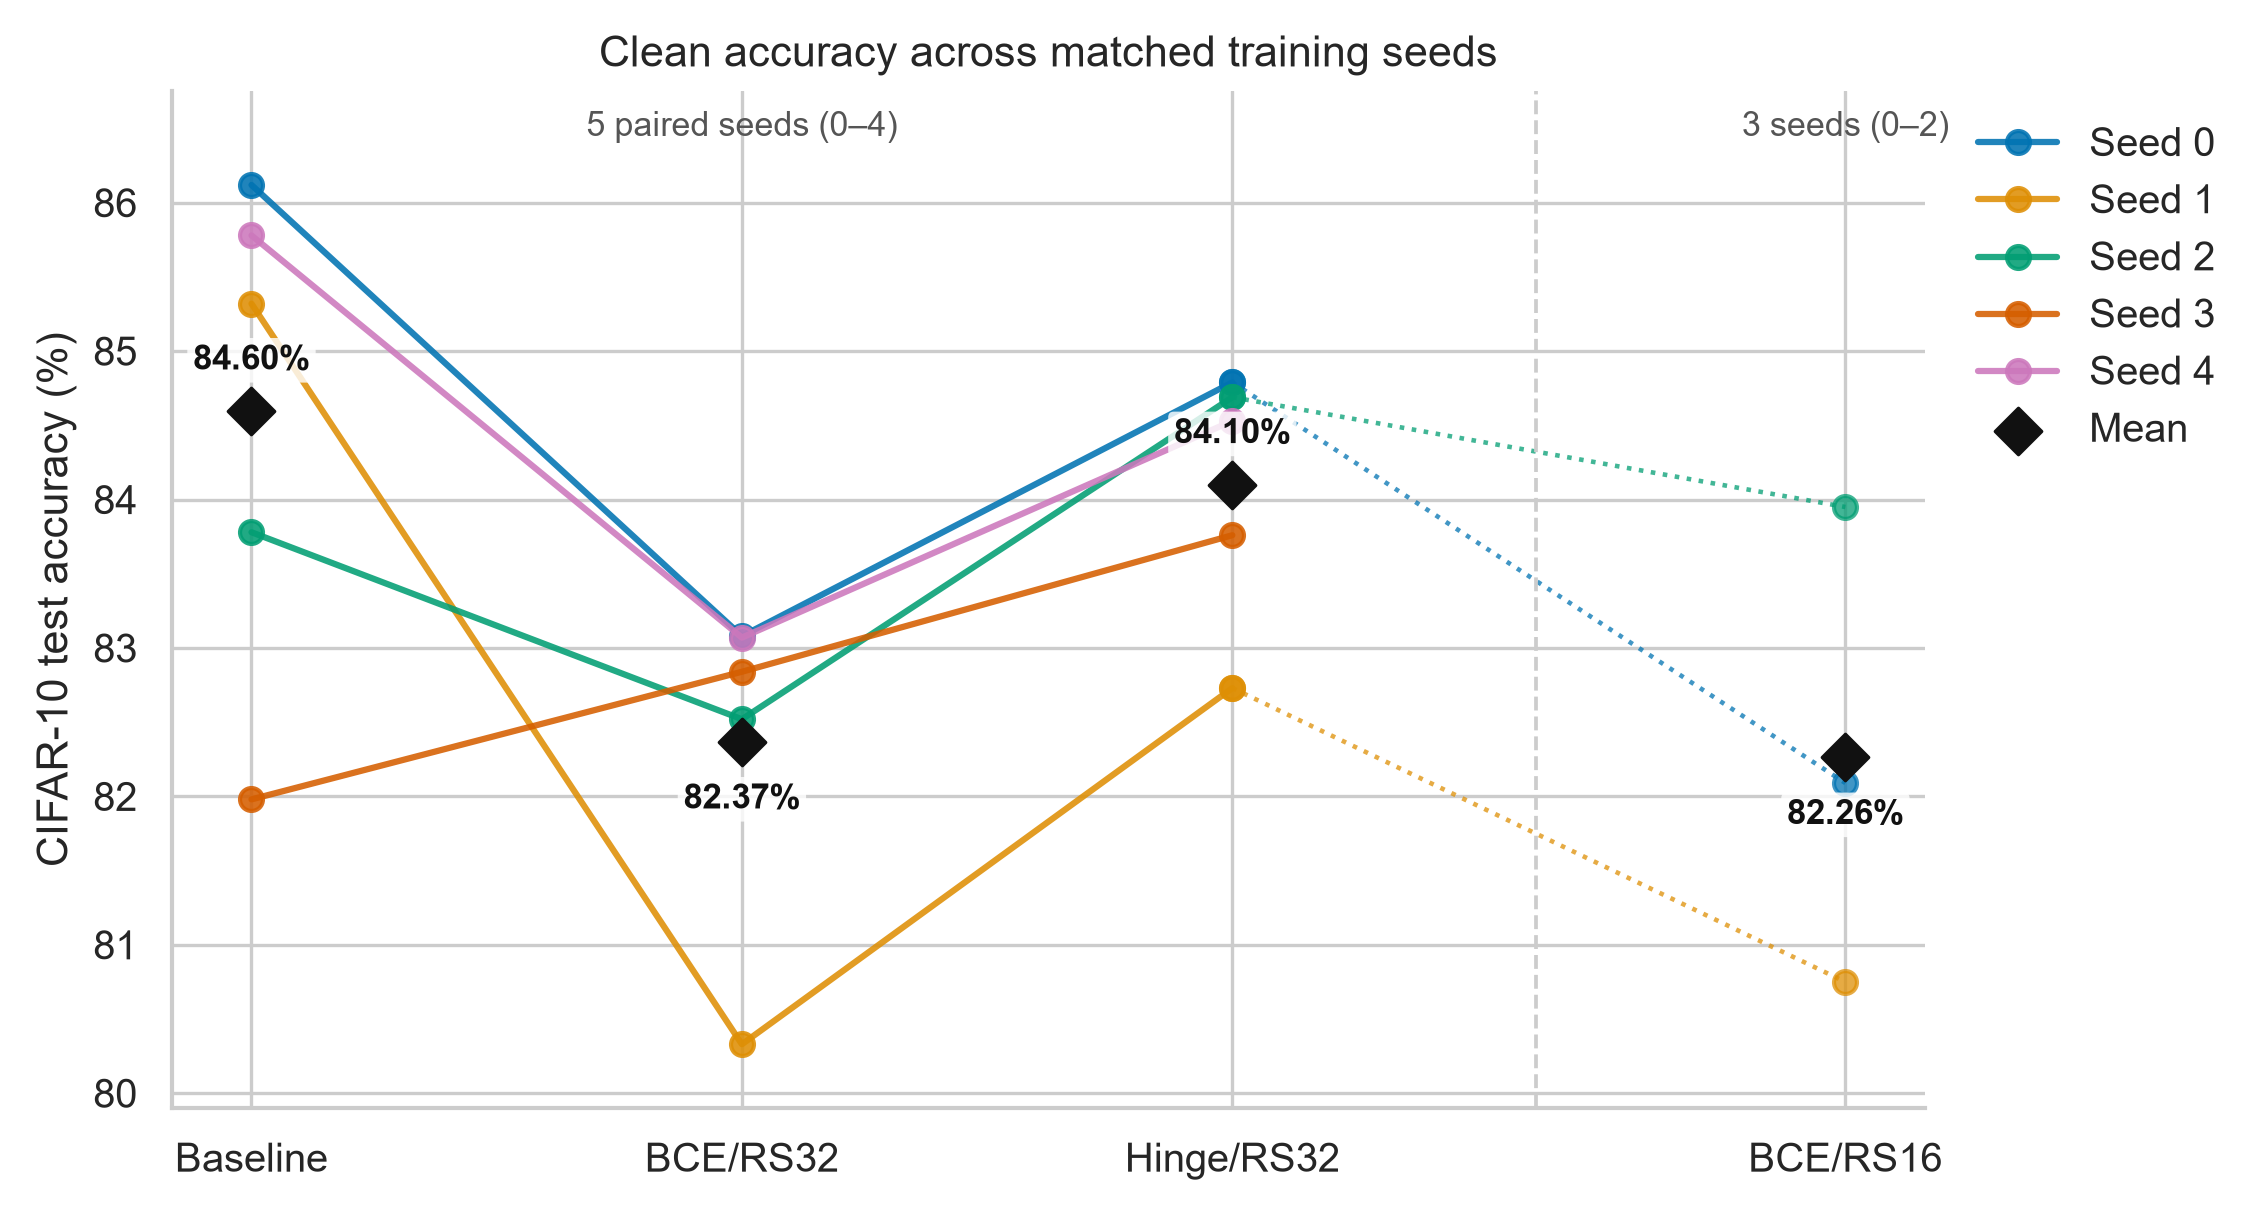
\includegraphics[width=\columnwidth]{figures/01_paired_accuracy.png}
\caption{Clean CIFAR-10 accuracy across paired training seeds. Hinge/RS32 uses $m=1.5$. BCE/RS16 is available for seeds 0--2.}\label{fig:accuracy}
\end{figure}

Table~\ref{tab:weight-split} and Fig.~\ref{fig:mechanism} describe the carrier rather than a causal mechanism. For $W$ with 128 flattened filters, shared energy is $128\|v\|_2^2/\|W\|_F^2$ and the residual norm is the mean across filters of $\|W_j-v\|_2$. Across seeds 0--2 the shared norm was about 5.05 for BCE/RS32 and 2.39 for hinge/RS32, with shared energy about 97\% and 88--89\%, respectively. The minimum absolute logit across the saved clean runs for each main design was 2.24 for BCE/RS32, 2.70 for BCE/RS16, and 1.50 for hinge/RS32. These measurements document differences accompanying the loss choice. They do not isolate the role of the shared norm or margin in either accuracy or overwrite resistance.

\begin{figure*}[!t]
\centering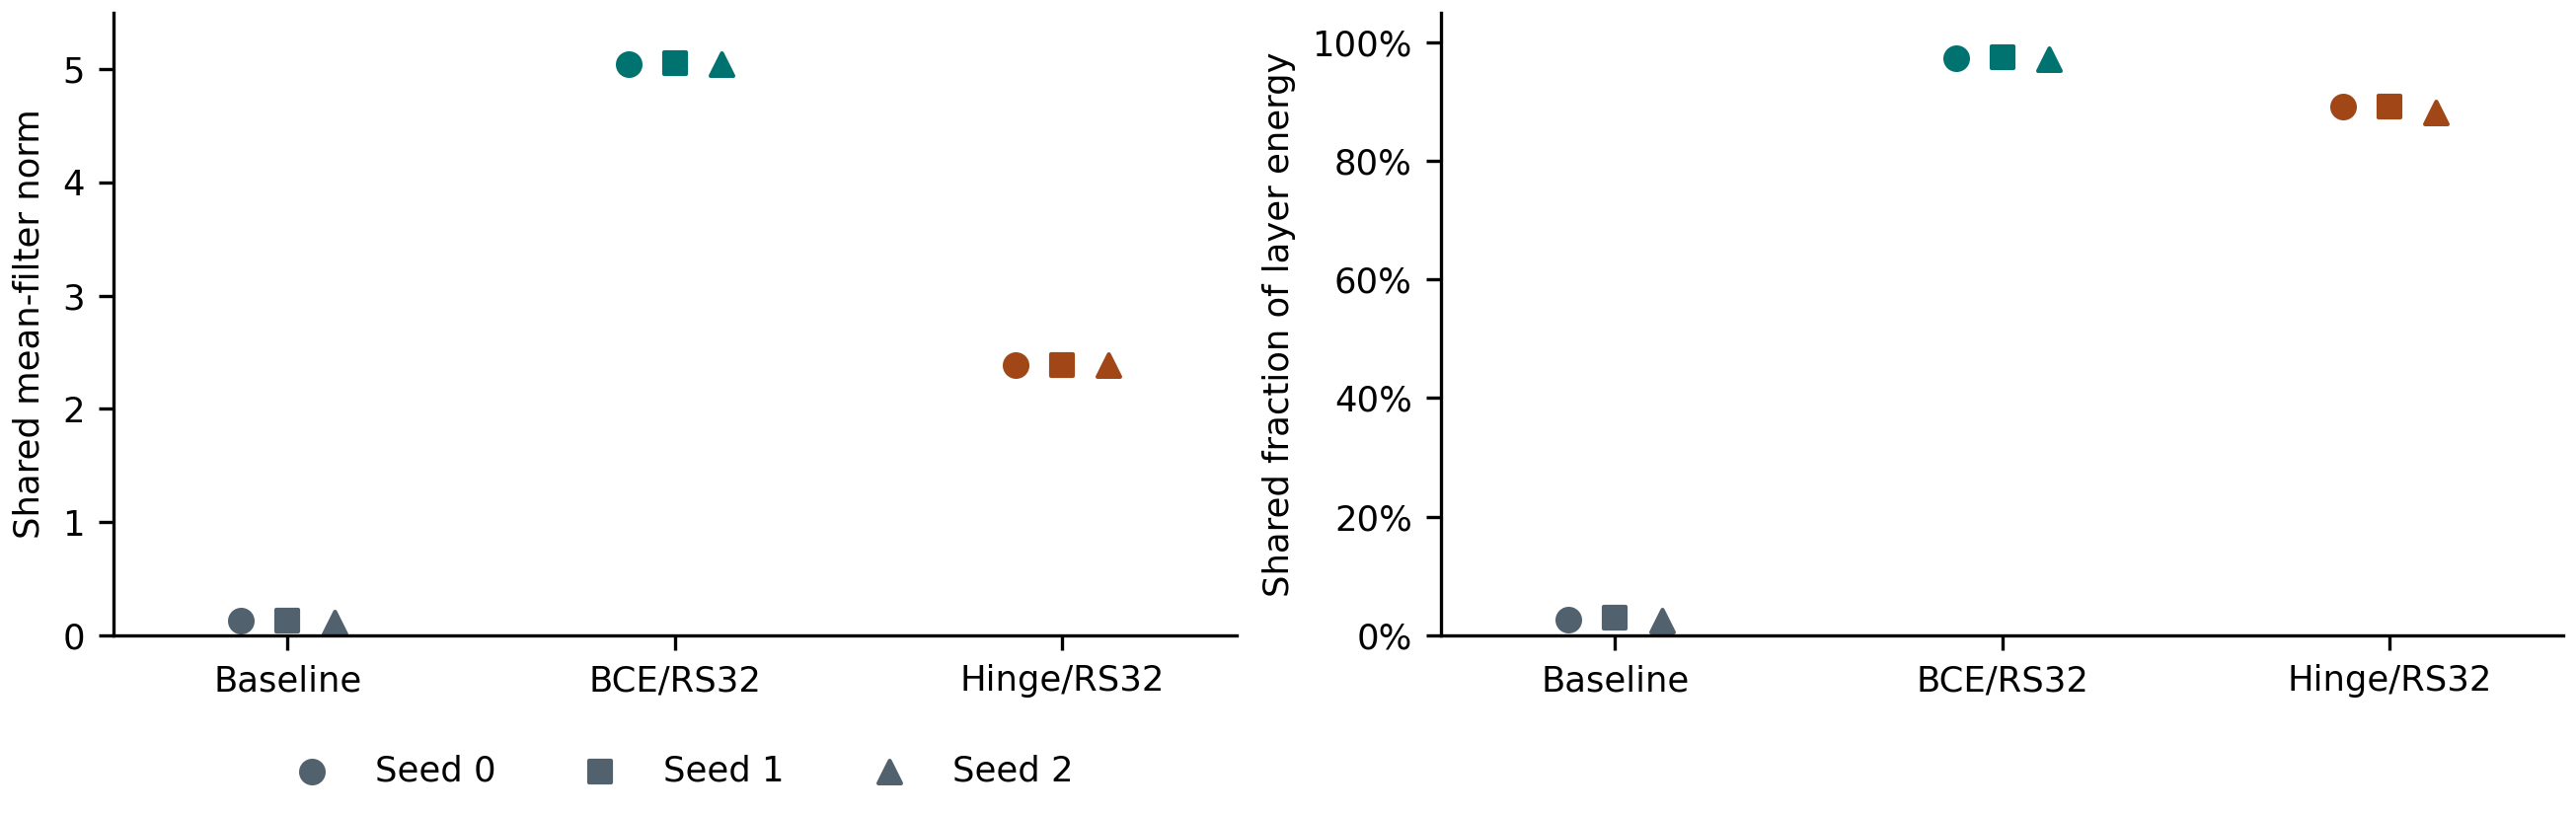
\includegraphics[width=0.90\textwidth]{figures/06_mechanism_bce_vs_hinge.png}
\caption{Carrier decomposition recomputed from the saved checkpoints for seeds 0--2. Each point is a trained model. Panels show the shared mean-filter norm and the fraction of layer energy in that mean.}\label{fig:mechanism}
\end{figure*}

\begin{table}[!t]
\centering
\caption{Carrier Decomposition, Seeds 0--2}
\label{tab:weight-split}
\footnotesize
\setlength{\tabcolsep}{3pt}
\begin{tabular}{@{}lrrrr@{}}
\toprule
Design & Shared & Residual & Ratio & Energy \\
\midrule
Baseline & 0.11--0.13 & 0.47--0.60 & 0.2 & 2--3\% \\
Hinge 1.5/RS32 & 2.39 & 0.57--0.67 & 3.6--4.2 & 88--89\% \\
Hinge 2.5 (seed 0) & 3.98 & 0.56 & 7.1 & 96\% \\
BCE/RS32 & 5.05 & 0.51--0.62 & 8.2--10.0 & 97\% \\
\bottomrule
\end{tabular}
\end{table}

At seed 0, the BCE/RS32 strength sweep used $\lambda=1,5,20$. The corresponding minimum absolute logits were 0.02, 1.21 and 2.25, with clean accuracies of 84.67\%, 83.19\% and 83.08\% (Fig.~\ref{fig:strength}). These are three recorded runs at one seed.

\begin{figure}[!tb]
\centering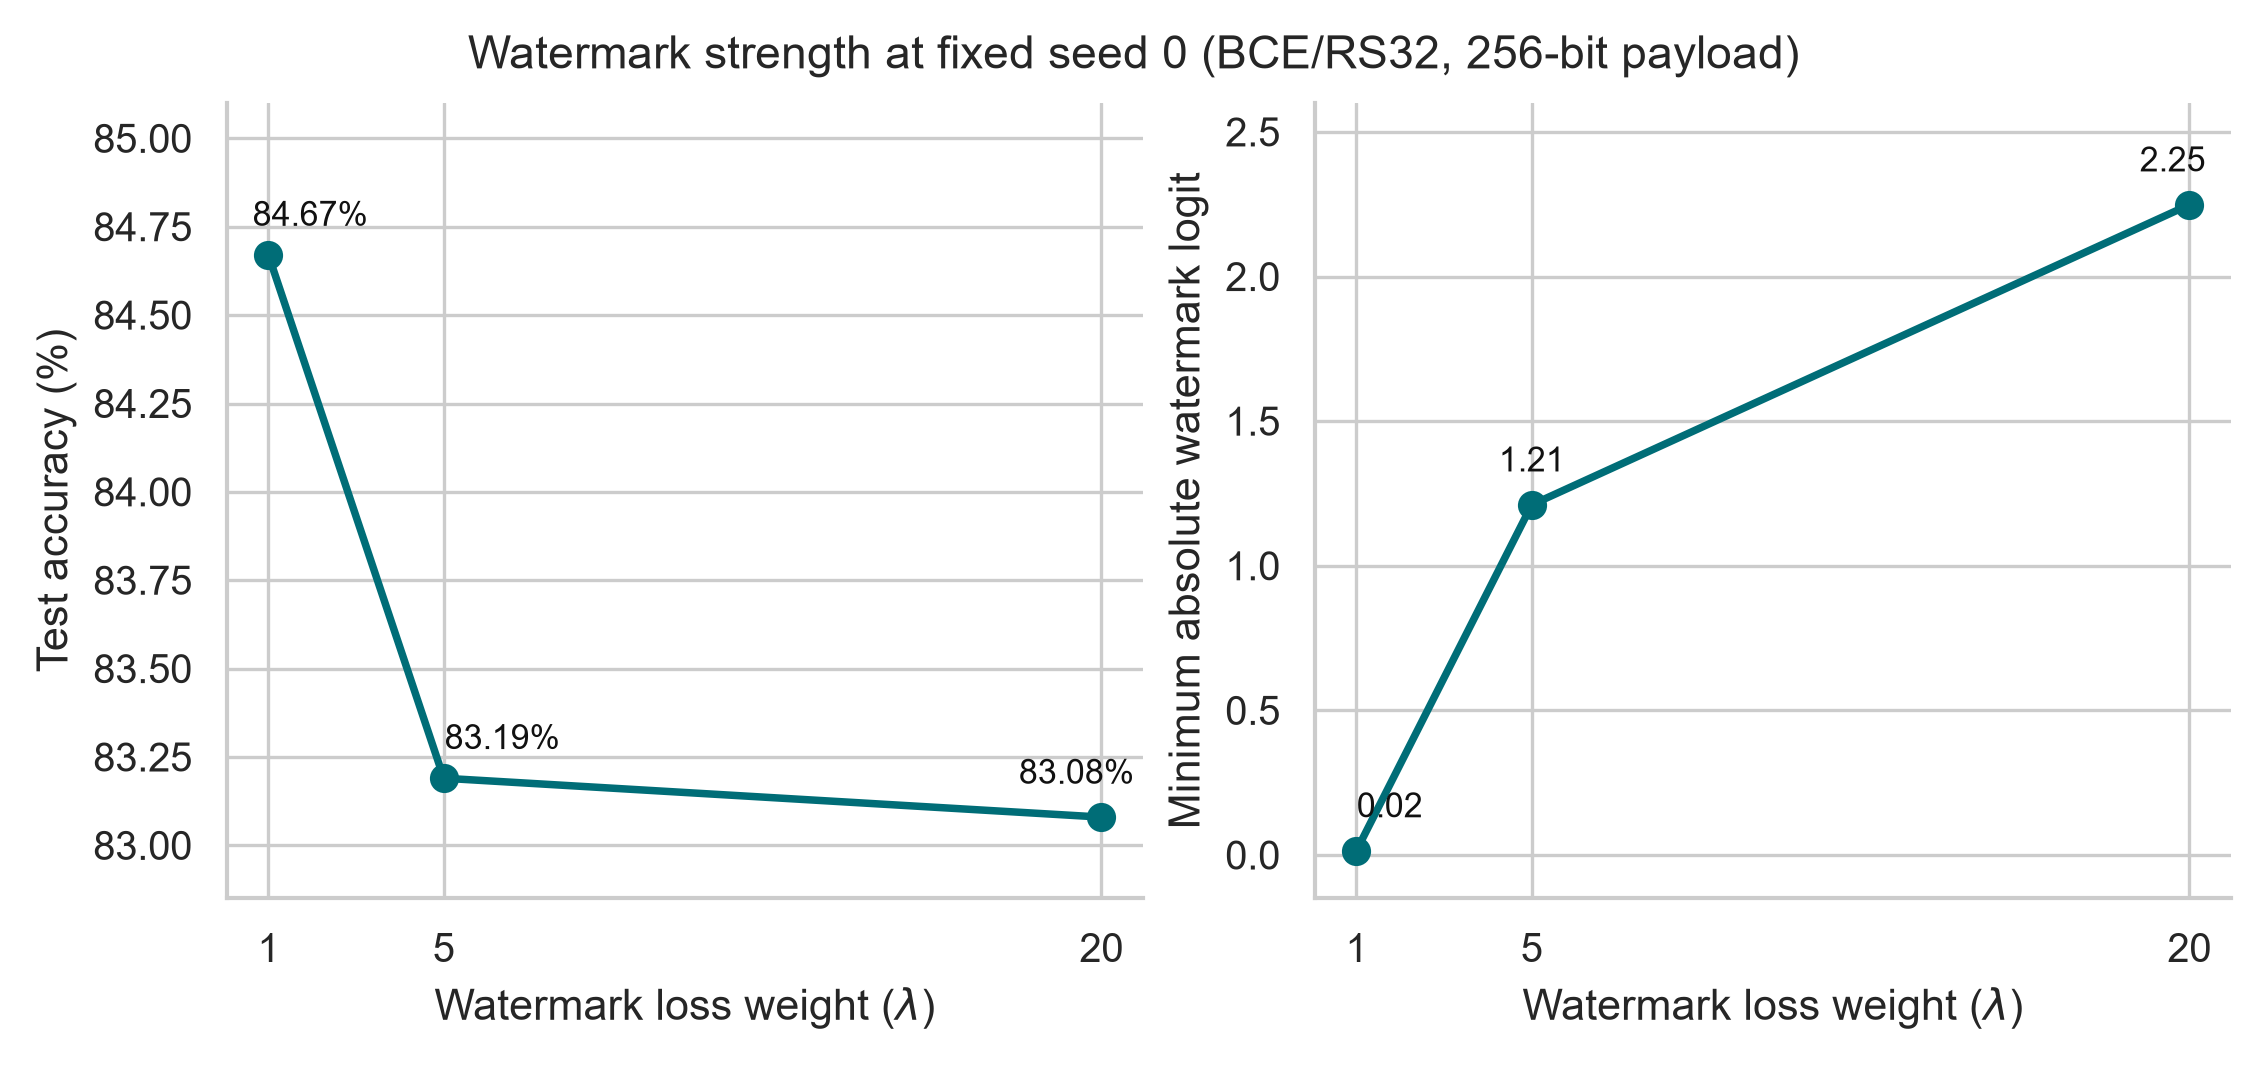
\includegraphics[width=\columnwidth]{figures/03_strength_seed0.png}
\caption{Strength sweep at fixed seed 0, carrier layer, BCE loss and 256-bit payload with RS32.}\label{fig:strength}
\end{figure}

\subsection{Verification, Utility, and Overwrite}
Table~\ref{tab:robustness} and Fig.~\ref{fig:robust} summarize saved verdicts. Exact recovery occurred even on checkpoints with large accuracy losses. For example, all three BCE/RS32 checkpoints verified after 70\% global pruning (mean accuracy 16.48\%) and after 3-bit per-tensor quantization (24.41\%). At 3 bits, the raw sign-change rate relative to the clean checkpoint averaged 1.11\%, hard RS decoding corrected 5.33 bytes on average with zero erasures on all three evaluations, and accuracy fell by 57.57 points on average (Fig.~\ref{fig:ecc}). At 2 bits, the three BCE/RS32 evaluations averaged 9.53\% accuracy. The rejected checkpoint scored 8.58\%.

Across the three designs, all 108 evaluations of output, input, or all-layer permutations and the combined permutation with $\times10$ input scaling verified. All 81 evaluations of input scaling alone also verified. Recorded test accuracy was unchanged in these 189 cases. All 81 separate output-side rescaling evaluations verified, with recorded accuracy changes of up to 0.07 points in absolute value. Figure~\ref{fig:align}A displays recorded structural results from the verifier with retries available. The figure does not estimate how many would verify with retries disabled.

\begin{table}[!t]
\centering
\caption{Saved Verdicts Across 252 Evaluations per Design}
\label{tab:robustness}
\footnotesize
\setlength{\tabcolsep}{3pt}
\begin{tabular}{@{}lrrrr@{}}
\toprule
Design & Verified & Damaged & Rejected & Removals \\
\midrule
BCE/RS32 & 231 & 20 & 1 & 0 \\
BCE/RS16 & 240 & 12 & 0 & 0 \\
Hinge/RS32 & 233 & 13 & 6 & 3 \\
\bottomrule
\end{tabular}
\end{table}

\begin{figure*}[!t]
\centering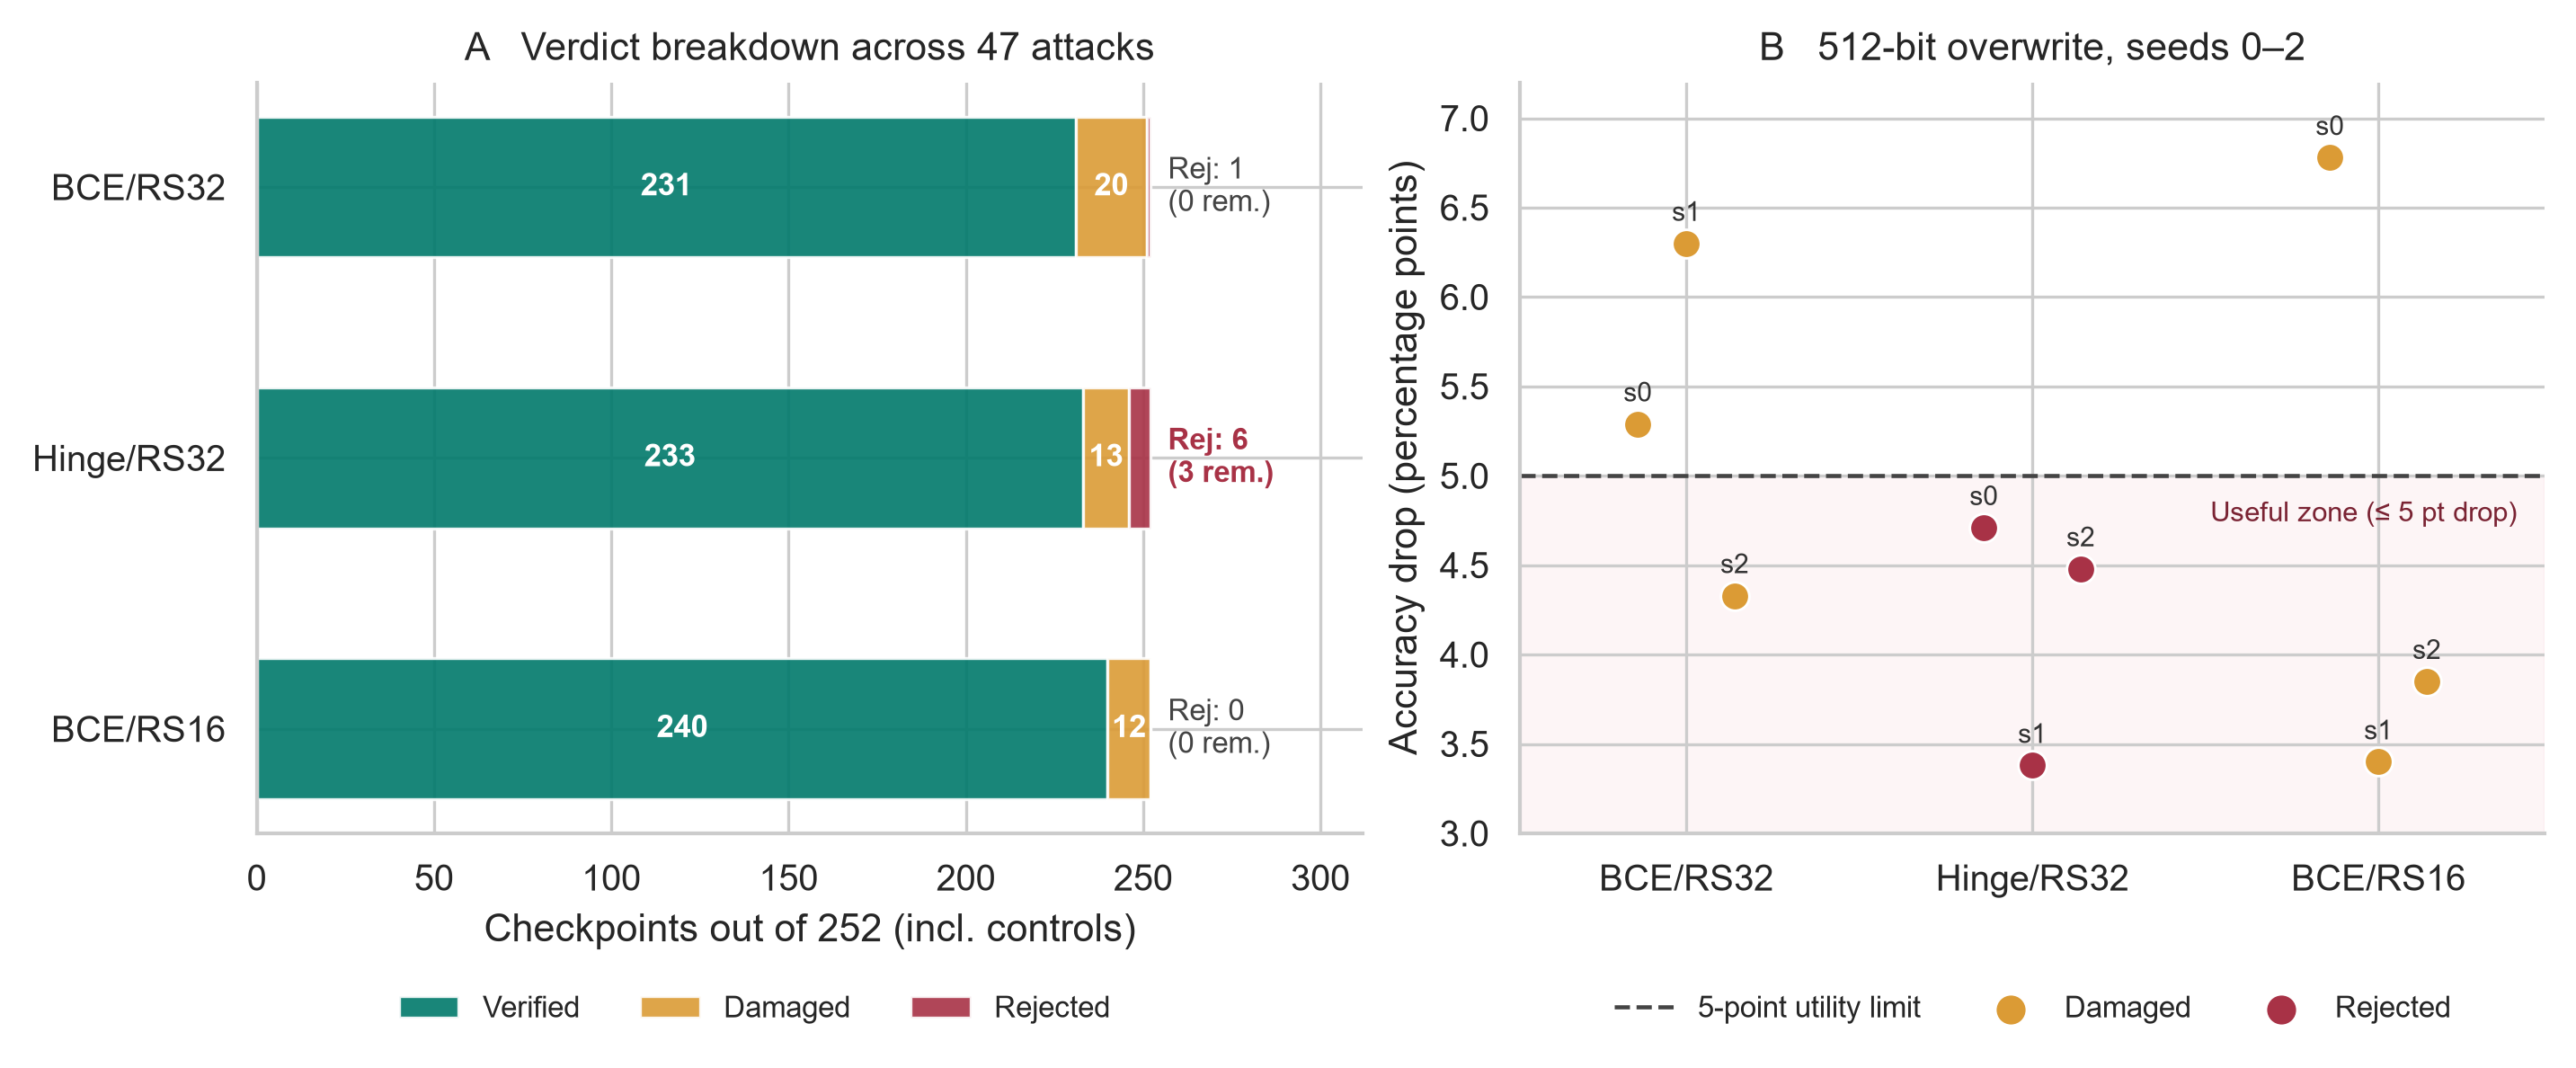
\includegraphics[width=0.90\textwidth]{figures/02_robustness.png}
\caption{Left: verdict counts, including three clean controls per design. Right: per-seed accuracy drop and verdict under a 512-bit same-layer overwrite. The three hinge rejections meet the five-point budget. All six BCE evaluations yield \textsc{Damaged}, including three within that budget.}\label{fig:robust}
\end{figure*}

Applying the utility filter row by row, the numbers of \textsc{Verified} evaluations within five points were 179, 181 and 184 for BCE/RS32, BCE/RS16 and hinge/RS32, respectively (176, 178 and 181 excluding their clean controls). In the 512-bit overwrite setting, hinge was rejected at drops of 4.71, 3.38 and 4.48 points, with 32.4--36.3\% of raw signs changed relative to the clean checkpoint. The other three hinge rejections were at 2-bit quantization (mean accuracy 9.90\%). The 512-bit BCE results were all \textsc{Damaged}. Their raw sign-change ranges were 20.3--25.0\% for RS32 and 15.9--24.2\% for RS16. One RS32 and two RS16 evaluations met the accuracy budget. Under the 128-bit overwrite, BCE/RS16 verified exactly in all three trials. There were zero successful removals for either BCE design in the recorded suite. Although hinge returned more exact matches than BCE/RS32 overall, the utility-filtered rejections expose an overwrite tradeoff.

\begin{figure}[!tb]
\centering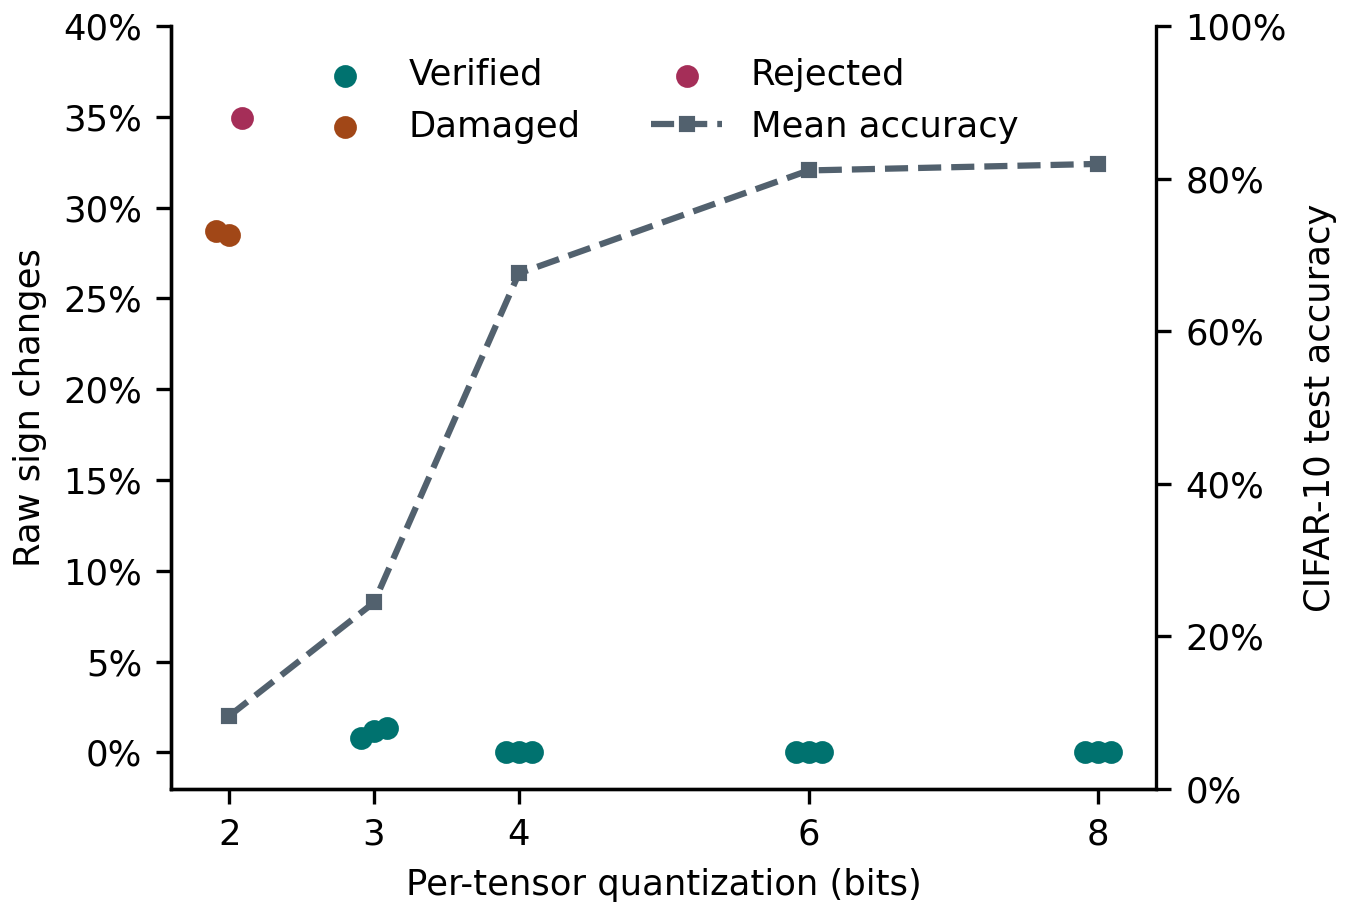
\includegraphics[width=\columnwidth]{figures/05_ecc_quantization.png}
\caption{BCE/RS32 per-tensor quantization across three seeds. The 3-bit checkpoints verified with byte corrections and zero erasures. At 2 bits, the mean accuracy was 9.53\% and the verdicts were two \textsc{Damaged} and one \textsc{Rejected}.}\label{fig:ecc}
\end{figure}

\subsection{RS32 Controls and Auxiliary Baseline}
We observed zero exact or residual detections in 724 RS32 extraction controls and zero in 54 attacked unmarked baseline evaluations (Table~\ref{tab:fp}). The extraction study includes 600 wrong-key trials on three marked checkpoints, and reuses checkpoints in several other groups. Its maximum recorded raw agreement was 305 of 512 (Fig.~\ref{fig:null}). The 54 attacked baselines are a separate cohort with saved verifier verdicts. These observations are specific to the sampled cases. They do not estimate the false-accept probability for an adaptive adversary or for RS16.

\begin{table}[!t]
\centering
\caption{RS32 Negative Controls}
\label{tab:fp}
\footnotesize
\setlength{\tabcolsep}{3pt}
\begin{tabular}{@{}lrrrr@{}}
\toprule
Cohort & Cases & False V/D & Mean & Max. \\
\midrule
Wrong watermark key & 600 & 0/0 & 256.2 & 305 \\
Unmarked baseline & 3 & 0/0 & 253.3 & 256 \\
Scrambled baseline & 15 & 0/0 & 258.5 & 278 \\
Third-party model & 1 & 0/0 & 264.0 & 264 \\
Scrambled third-party & 5 & 0/0 & 259.2 & 265 \\
Random initialization & 100 & 0/0 & 256.1 & 289 \\
Attacked baseline & 54 & 0/0 & --- & --- \\
\midrule
Total & 778 & 0/0 & --- & --- \\
\bottomrule
\end{tabular}
\end{table}

\begin{figure}[!tb]
\centering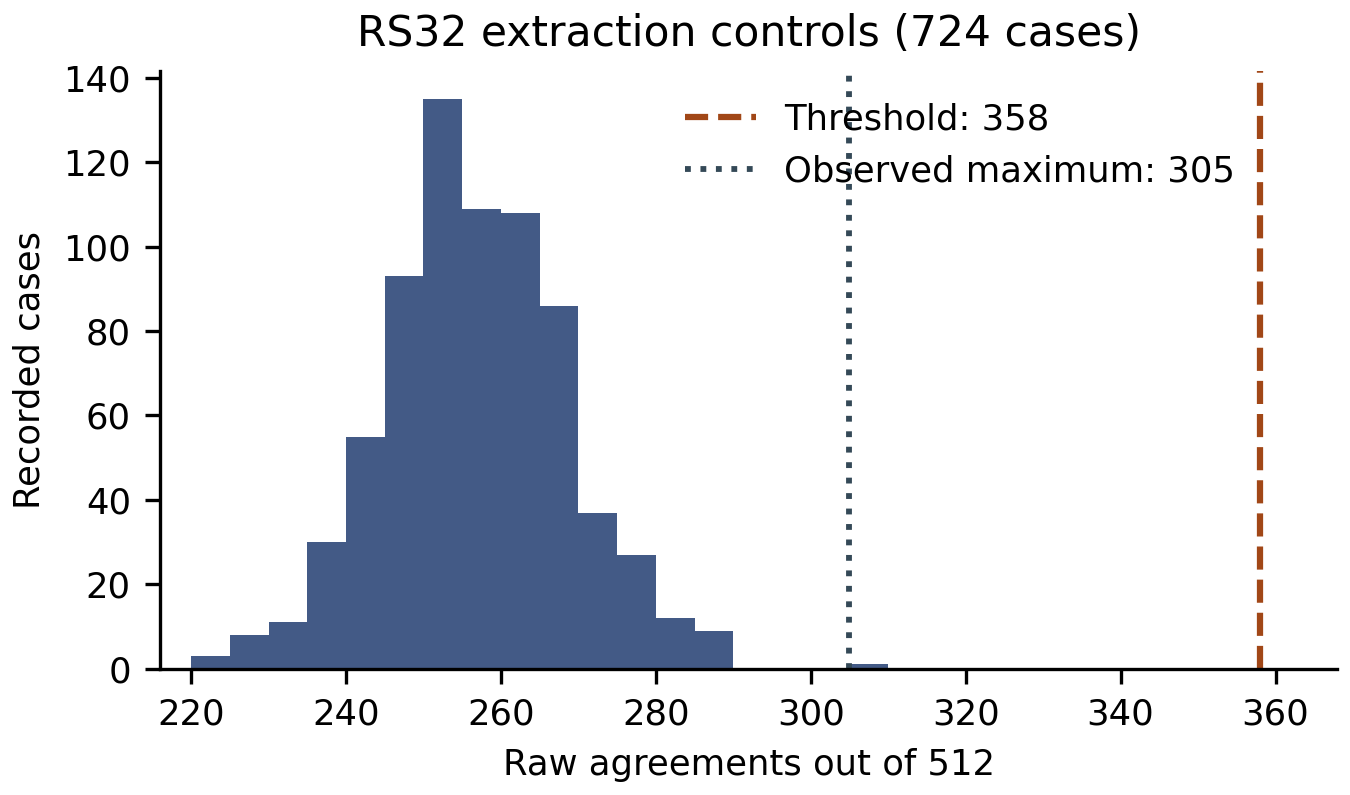
\includegraphics[width=\columnwidth]{figures/04_false_positive_controls.png}
\caption{Observed raw agreement across the 724 RS32 extraction controls. The vertical line marks the decision threshold at 358 of 512. The separate attacked-baseline cohort is excluded.}\label{fig:null}
\end{figure}

An exploratory comparison assigns each RS32 bit to the sign of one keyed weight after training (Fig.~\ref{fig:align}B). The naive mark reduced clean accuracy by 0.09 points on average across two seeds. It was removed within budget in six configurations. Averaging equally over the 36 common non-control weight-attack settings, the exact verification rates were 26\% for the naive method and 86\% for the BCE/RS32 projection pipeline. The combined exact-or-residual rates were 61\% and 99\%. The naive extractor has no alignment retry. It uses two seeds and one draw per stochastic setting, compared with three seeds and three draws for projection. These are descriptive pipeline comparisons.

\begin{figure*}[!t]
\centering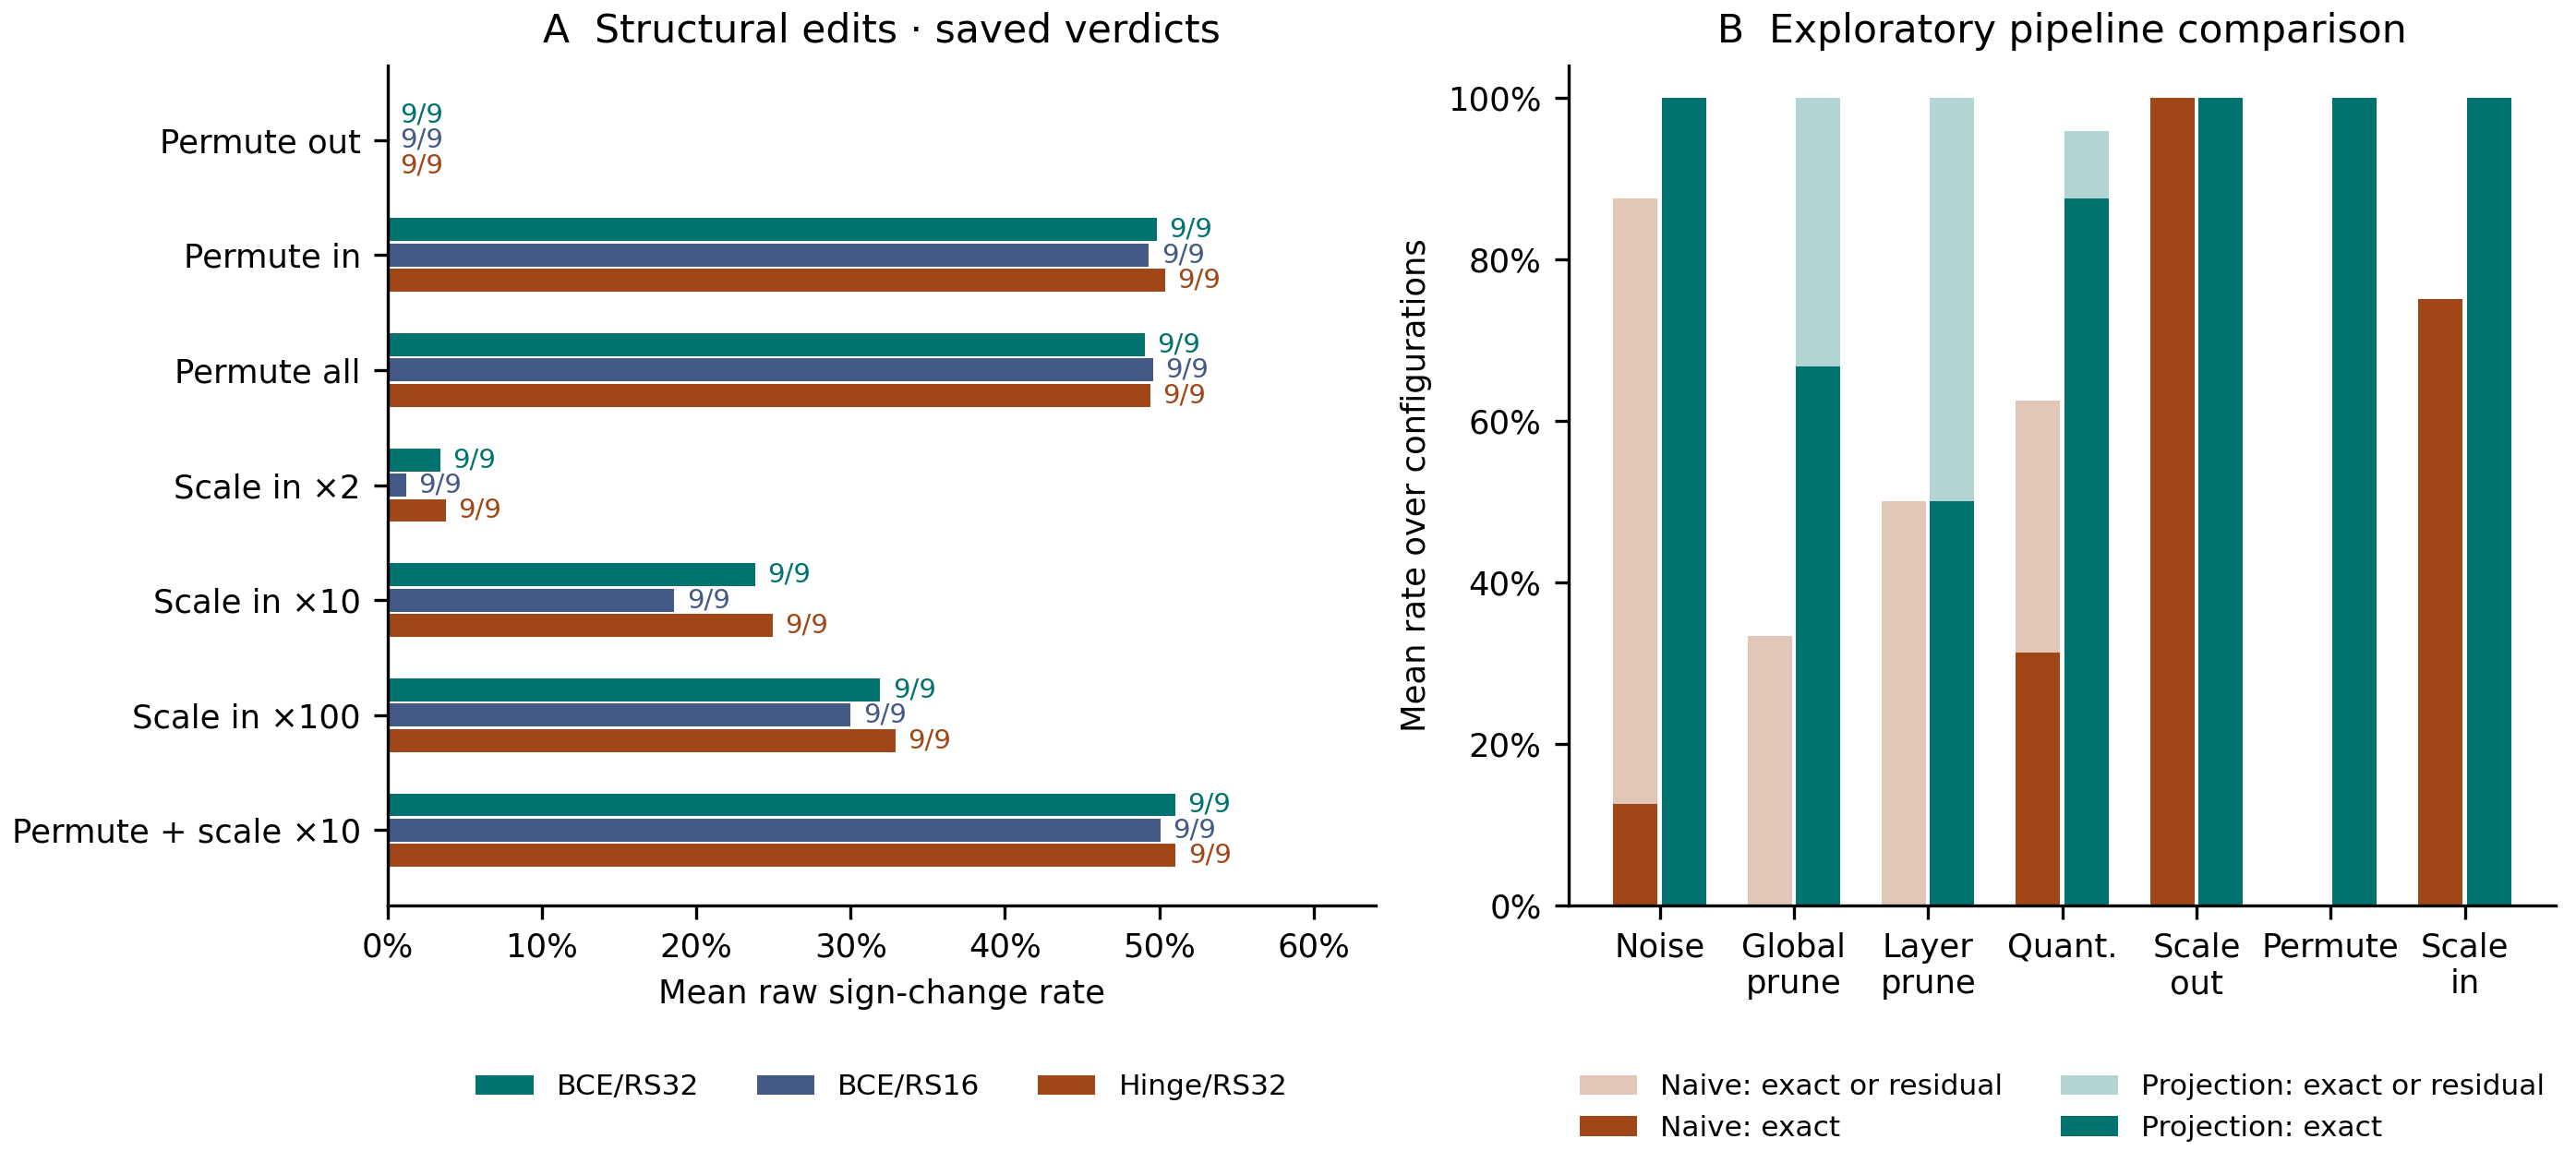
\includegraphics[width=0.96\textwidth]{figures/07_alignment_and_attacks.png}
\caption{(A) Mean raw sign changes relative to the clean checkpoints, with exact verdict counts from the verifier with retries available. Each configuration has nine recorded evaluations per design. (B) Recorded exact and exact-or-residual rates for the naive and projection pipelines, averaged equally across common configurations within each family. The baseline evaluation uses different seed and repeat counts.}\label{fig:align}
\end{figure*}

\section{Discussion and Conclusion}
\label{sec:conclusion}
In this \textsc{SmallCNN}/CIFAR-10 evaluation, changing from BCE to hinge with RS32 improved clean accuracy across the five paired runs. In the specified 512-bit overwrite, all three hinge checkpoints were rejected within the stated utility budget, while both BCE designs retained residual agreement in all tested repeats. The carrier measurements accompany these outcomes. Matched-margin and strength controls would be needed to assess whether either quantity accounts for the observed difference.

The benchmark uses one architecture, dataset, release and watermark key, and one overwrite draw per trained model at each setting. Longer fine-tuning, distillation, cross-layer overwrites and architecture-changing obfuscation remain untested. Smaller payloads and a matched no-ECC ablation remain open. We lack a matched alignment on/off evaluation for the structural suite. The fixed-order strict-fit count and the one-shot raw-agreement null have distinct assumptions. A false-accept analysis for the complete retry and decoder remains open. The trusted auditor setting also leaves key distribution and revocation as operational questions.

The prototype uses a standardized post-quantum signature for manifest authenticity and evaluates an error-corrected weight association separately. Reporting exact recovery, residual agreement and classifier utility together makes the observed clean-accuracy and overwrite tradeoff visible.
